%%% Afin d'obtenir de meilleurs performances avec PostgreSQL, dans la
%%% plupart des cas, l'approche la plus efficace consiste à revoir la
%%% manière dont le SQL est écrit. Et pour écrire un SQL plus rapide,
%%% souvent, la meilleure approche consiste à revoir le schéma de données…
%%%
%%% Cette présentation donne quelques trucs et astuces afin d'obtenir de
%%% meilleures performances, mais pas à n'importe quel prix !

\documentclass{beamer}

\usepackage{minted}
%% \usemintedstyle{emacs}
\usepackage{beamerthemesplit}
\usepackage[utf8]{inputenc}
%% \usetheme{AnnArbor}
\usetheme{Boadilla}
%% \usetheme{Pittsburgh}
%% \usecolortheme{beaver}
\beamertemplatetransparentcovered

\title{The Need For Speed}
\subtitle{leads to PostgreSQL}
\author{Dimitri Fontaine \url{dimitri@2ndQuadrant.fr}}
\date{28 Mars 2013}
\logo{
\includegraphics[height=0.4cm]{2ndQuadrant-cross.png}}

\begin{document}

\frame{\titlepage}

\section{Introduction}

\begin{frame}[fragile]
  \frametitle{Dimitri Fontaine}

  \begin{center}
    \textbf{2ndQuadrant France}
    \linebreak
    PostgreSQL Major Contributor
  \end{center}
  \vfill

\begin{columns}[c]
\column{.75\textwidth} 

  \begin{itemize}
   \item<1-> \texttt{pgloader}, \texttt{prefix}, \texttt{skytools}, \texttt{debian}, …
   \item<1-> \texttt{\textbf{CREATE EXTENSION}}
   \item<2-> \texttt{\textbf{CREATE EVENT TRIGGER}}
   \item<3-> \textit{Bi-Directional Réplication}
   \item<4-> \textit{Partitionnement}
  \end{itemize}  

\column{.25\textwidth}
\begin{center}
  
\includegraphics[height=5em]{bulle-blue-icon.png}
\end{center}
\end{columns}
\end{frame}

\begin{frame}[fragile]
  \frametitle{Optimisation SQL}

  \center{Quelques expériences d'optimisations}
  \vfill

\begin{columns}[c]
\column{.6\textwidth} 

  \begin{itemize}
  \item Optimisation de requêtes
  \item Migration Oracle, de 1h30 à 5mins
  \item \texttt{prefix}, \textit{GiST indexing}
  \item \texttt{pgloader}
  \item \texttt{preprepare}
  \end{itemize}

\column{.4\textwidth}
\begin{center}
  
\includegraphics[height=5em]{Dollar-sign.jpg}
\end{center}
\end{columns}
\end{frame}

\begin{frame}[fragile]
  \frametitle{Extract Month From date, THE HORROR}

  \center{Certaines requêtes \texttt{SQL} sont assez faciles à optimiser.}
  \vfill

\begin{minted}{postgresql}
select f1, f2, f3, d
  from table t
 where   extract('month' from t.d)
       = extract('month' from now());
\end{minted}
\end{frame}

\section{Why}

\begin{frame}[fragile]
  \frametitle{Performance Club}

  \center{\url{http://fetter.org/optimization.html}}
  \vfill

\begin{columns}[c]
\column{.75\textwidth} 

  \begin{enumerate}
  \item<1-> The first rule of Optimization is, you do not talk about Optimization.
  \item<1-> The second rule of Optimization is, you \textbf{DO NOT} talk about
    Optimization.
  \item<2-> If your app is running faster than the underlying transport
    protocol, the optimization is over.
  \item<2-> One factor at a time.
  \item<2-> No marketroids, no marketroid schedules.
  \item<3-> Testing will go on as long as it has to.
  \item<4-> If this is your first night at Optimization Club, you have to
    write a test case.
  \end{enumerate}


\column{.25\textwidth}
\begin{center}
  
\includegraphics[height=5em]{performanceClubPromo.jpg}
\end{center}
\end{columns}
\end{frame}

\begin{frame}
  \frametitle{Diminishing Returns}

  \center{Loi des rendements décroissants}
  \vfill

\begin{columns}[c]
\column{.6\textwidth} 

  \begin{itemize}
  \item \textit{Plus tu pédales moins vite, moins plus vite tu avances}
  \item Maîtriser l'effort d'optimisation
  \item Difficulté de savoir quand on est allé assez loin
  \item Prendre du recul sur ce que l'on fait
  \end{itemize}

\column{.4\textwidth}
\begin{center}
  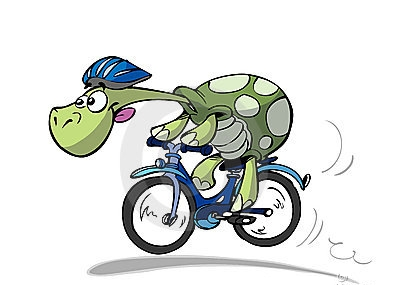
\includegraphics[height=7em]{cartoon-velo.jpg}
\end{center}
\end{columns}
\end{frame}

\begin{frame}
  \frametitle{Qualité de service}

  \center{La performance de cette requête SQL a-t'elle un impact clair sur
    la qualité de service offerte à vos clients ?}

\begin{columns}[c]
\column{.6\textwidth} 

  \begin{itemize}
    \item \textit{A one second delay in page-load can cause 7\% loss in customer conversions}
    \item \url{http://econsultancy.com/fr/blog/10936-site-speed-case-studies-tips-and-tools-for-improving-your-conversion-rate}
    \item \textit{If you make \$1,000 a month from your site — that’s seventy bucks a month you are losing — and \$840 a year. Can you afford to just throw away \$70 a month? \$840 a year?}
    \item \url{http://www.copyblogger.com/website-speed-matters/}
  \end{itemize}

\column{.4\textwidth}
\begin{center}
  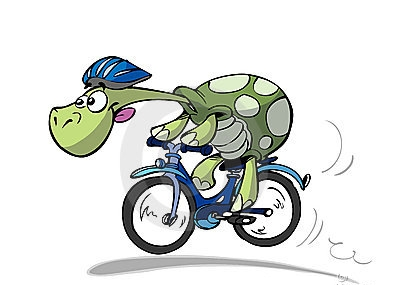
\includegraphics[height=7em]{cartoon-velo.jpg}
\end{center}
\end{columns}
\end{frame}

\section{What}

\begin{frame}
  \frametitle{La performance c'est quoi ?}

  \center{Améliorer les performances ne peut se faire qu'après avoir
    \textit{profilé}}
  \vfill

\begin{columns}[c]
\column{.3\textwidth} 

  \begin{itemize}
  \item Loi d'Amdahl
  \item \textit{profiling}
  \item \textit{metrologie}
  \end{itemize}

\column{.7\textwidth}
\begin{center}
  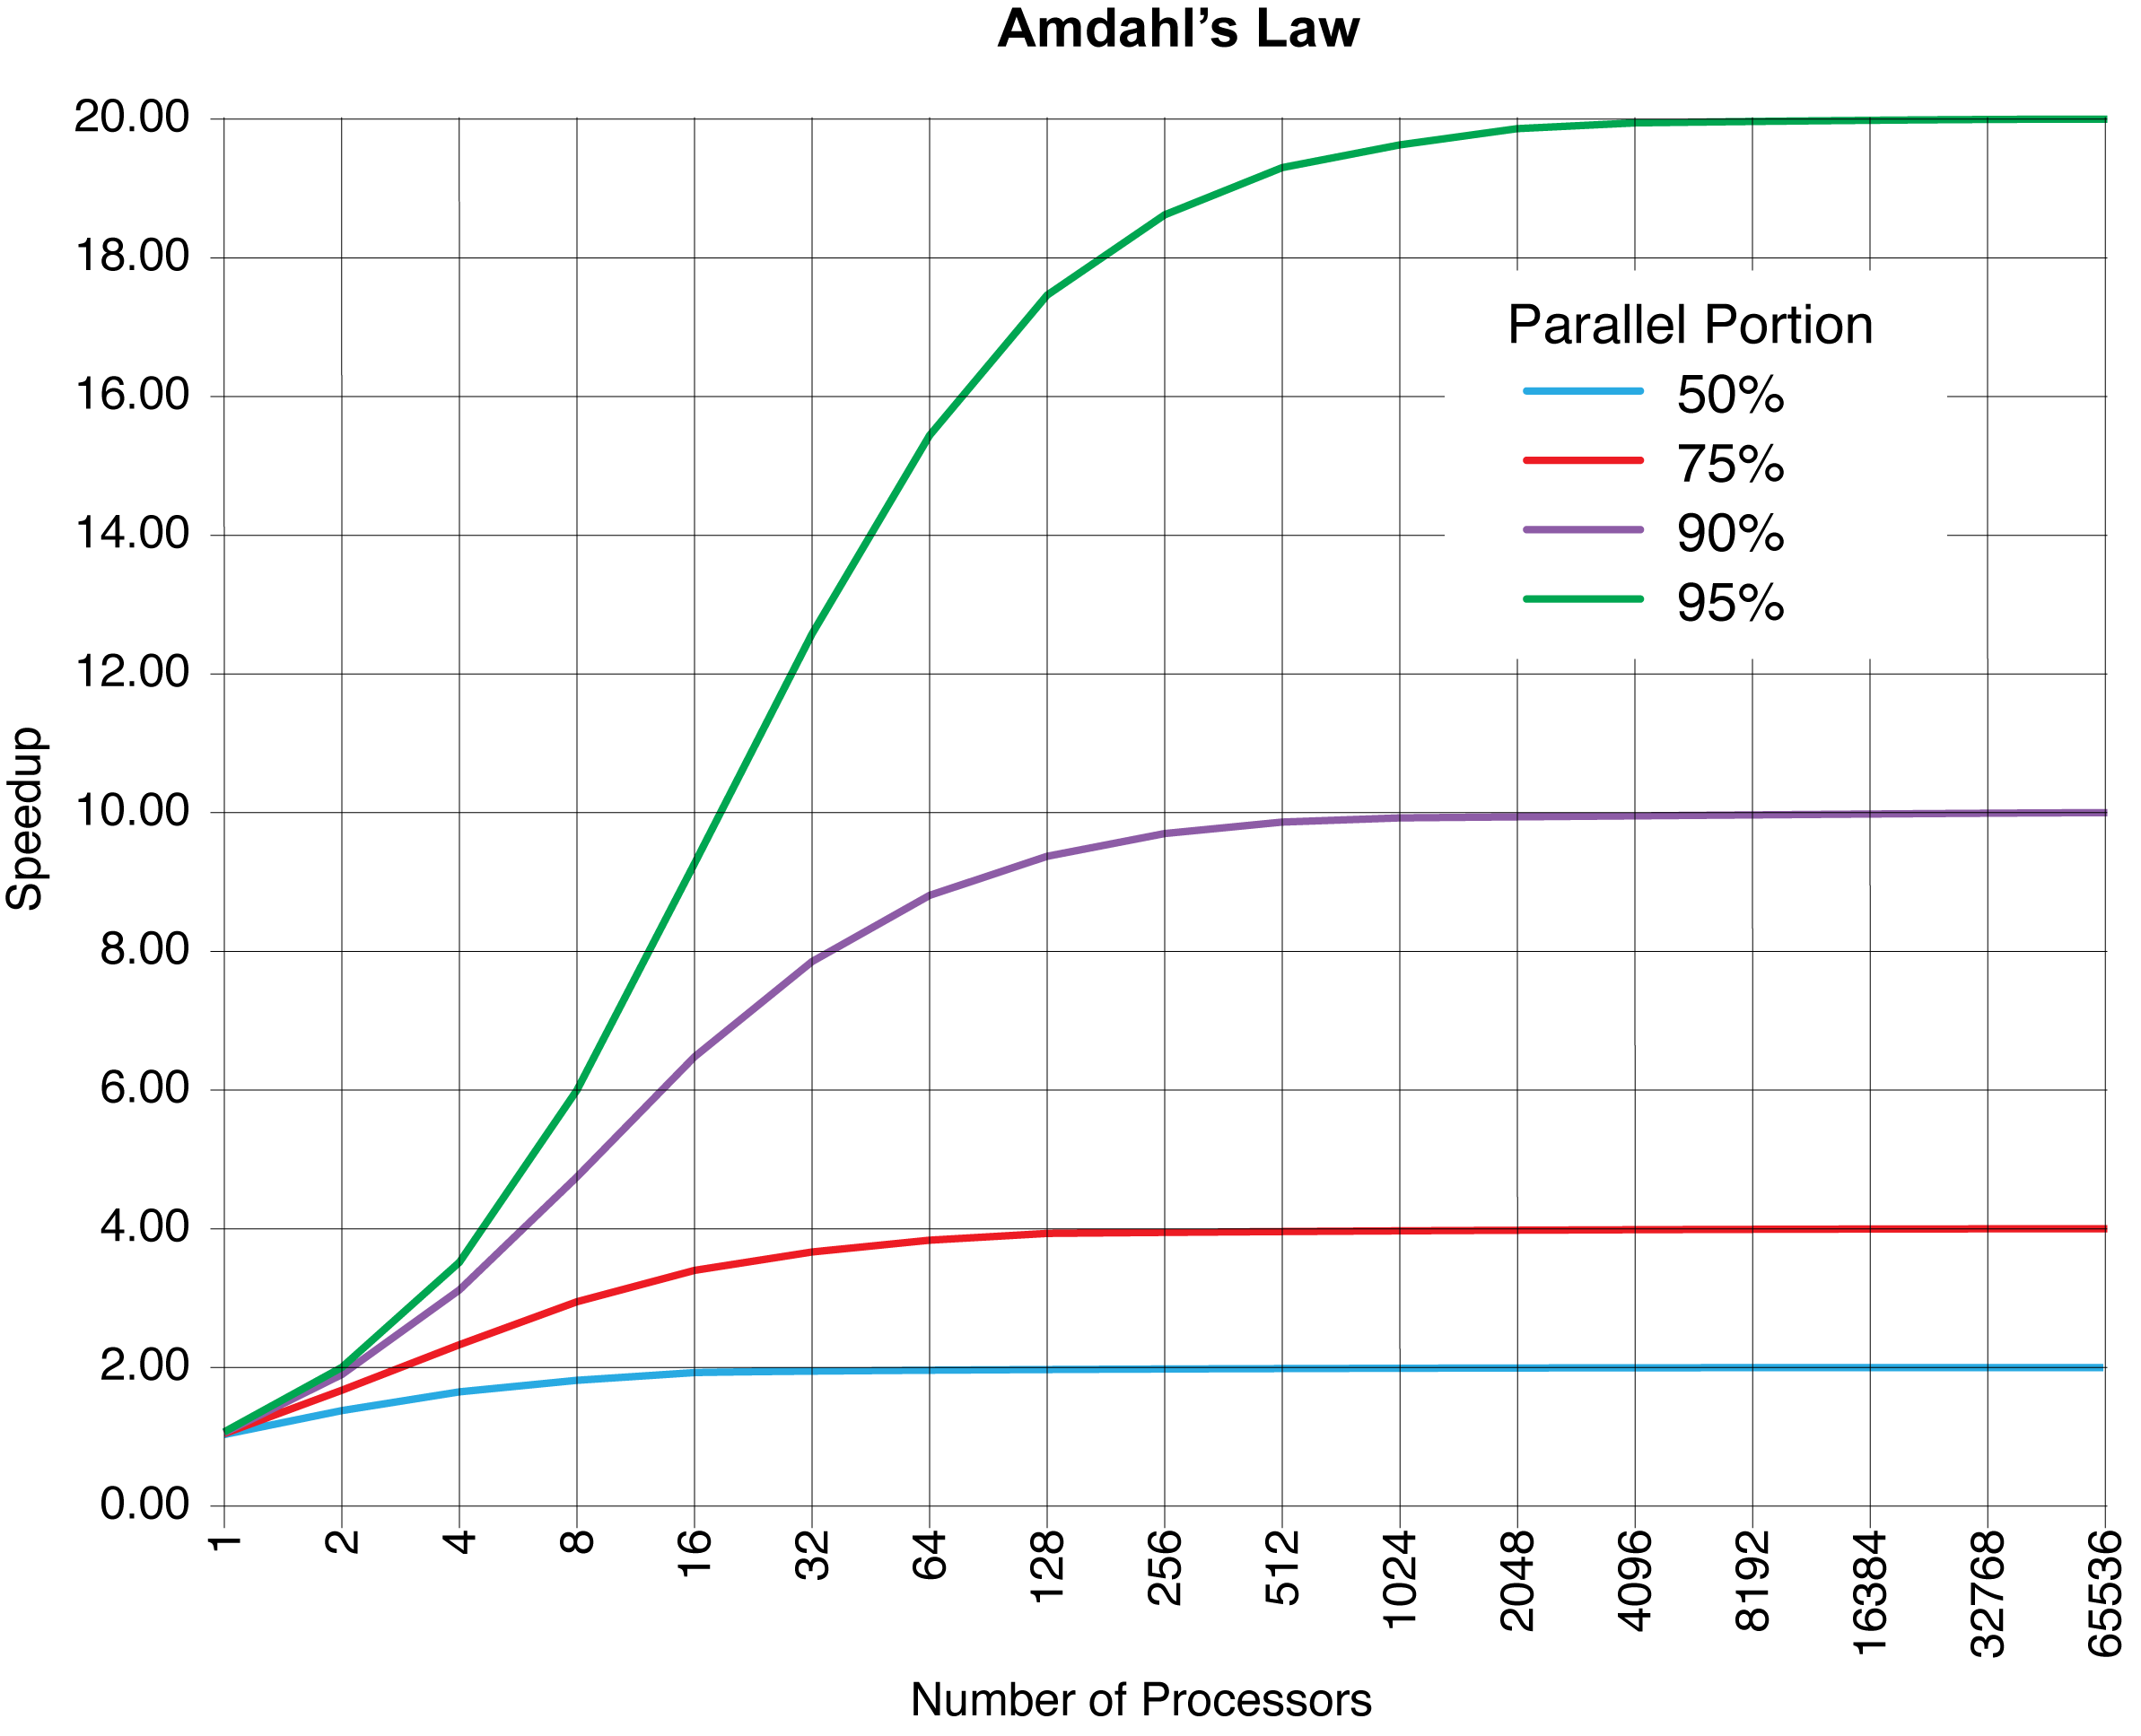
\includegraphics[height=16em]{amdahlslaw.png}
\end{center}
\end{columns}
\end{frame}

\begin{frame}
  \frametitle{La performance c'est quoi ?}

  \center{Mesurer les performances}
  \vfill

\begin{columns}[c]
\column{.7\textwidth} 

  \begin{itemize}
  \item \texttt{EXPLAIN}
  \item \texttt{EXPLAIN (VERBOSE, BUFFERS, ANALYZE)}
  \item \texttt{psql \\timing}
  \end{itemize}

\column{.3\textwidth}
\begin{center}
  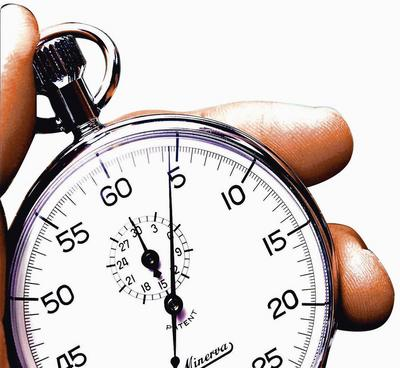
\includegraphics[height=9em]{timing.jpg}
\end{center}
\end{columns}
\end{frame}

\begin{frame}
  \frametitle{La performance c'est quoi ?}

  \center{Attention aux allers retours entre client et serveur}
  \vfill

\begin{columns}[c]
\column{.6\textwidth} 

  \begin{itemize}
  \item Round-trip
  \item Bande passante (\textit{bandwidth})
  \end{itemize}

\column{.4\textwidth}
\begin{center}
  
\includegraphics[height=5em]{roundtrip.png}
\end{center}
\end{columns}
\end{frame}

\section{When}

\begin{frame}
  \frametitle{La performance : quand s'y intéresser ?}

  \center{Premature optimization is the root of all evil}
  \vfill

\begin{columns}[c]
\column{.75\textwidth} 

In \textbf{Donald Knuth}'s paper \textit{Structured Programming with go to
  Statements} at
\url{http://pplab.snu.ac.kr/courses/adv_pl05/papers/p261-knuth.pdf}
\linebreak \vfill

Programmers waste enormous amounts of time thinking about, or worrying
about, the speed of noncritical parts of their programs, and these attempts
at efficiency actually have a strong negative impact when debugging and
maintenance are considered. We should forget about small efficiencies, say
about 97\% of the time: premature optimization is the root of all evil. Yet
we should not pass up our opportunities in that critical 3\%.

\column{.25\textwidth}
\begin{center}
  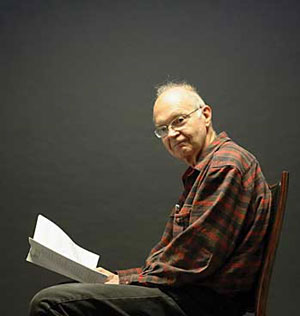
\includegraphics[height=7em]{knuth.jpg}
\end{center}
\end{columns}
\end{frame}

\begin{frame}
  \frametitle{La performance : quand s'y intéresser ?}

  \center{Premature optimization is the root of all evil}
  \vfill

\begin{columns}[c]
\column{.75\textwidth} 

\begin{itemize}
  \item Jamais trop tôt
  \item Avant qu'il ne soit trop tard
  \item Préparation d'une phase de croissance
  \item Réduction des dépenses énergétique
  \item Réduction de la facture d'hébergement
  \item Meilleur service aux utilisateurs
\end{itemize}

\column{.25\textwidth}
\begin{center}
  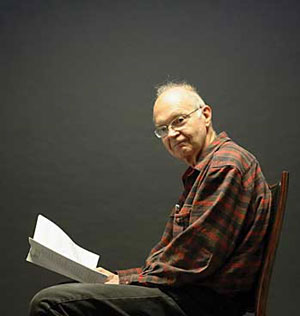
\includegraphics[height=7em]{knuth.jpg}
\end{center}
\end{columns}
\end{frame}

\section{How}

\begin{frame}
  \frametitle{Comment améliorer les performances}

  \center{Approche globale pour améliorer les performances}
  \vfill

\begin{columns}[c]
\column{.6\textwidth} 

\begin{itemize}
  \item Optimisation optimale : \textbf{ne pas} exécuter la requête !
  \item Traitements par lots (\textit{batch})
  \item Traitements hors lignes (\textit{asynchrone})
  \item \texttt{PGQ}
  \item \texttt{LISTEN} et \texttt{NOTIFY}
\end{itemize}

\column{.4\textwidth}
\begin{center}
  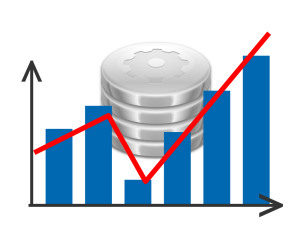
\includegraphics[height=10em]{optimisation.jpg}
\end{center}
\end{columns}
\end{frame}

\begin{frame}
  \frametitle{Outils d'anlyze des performances des requêtes 1/2}

  \center{Analyzer les performances}
  \vfill

\begin{columns}[c]
\column{.6\textwidth} 

\begin{itemize}
  \item \texttt{EXPLAIN}
  \item \texttt{(ANALYZE, VERBOSE, BUFFERS)}
  \item \texttt{INSERT, DELETE, UPDATE}
  \item \textit{(ne pas oublier de \texttt{ROLLBACK})}
\end{itemize}

\column{.4\textwidth}
\begin{center}
  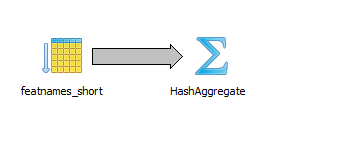
\includegraphics[height=8em]{pg91_btree_explain_like2.png}
\end{center}
\end{columns}
\end{frame}

\begin{frame}
  \frametitle{Outils d'anlyze des performances des requêtes 2/2}

  \center{Analyzer les performances}
  \vfill

\begin{columns}[c]
\column{.6\textwidth} 
\begin{itemize}
  \item \texttt{Nested Loops}
  \item \url{http://explain.depesz.com/}
  \item \texttt{SELECT * FROM pg\_locks;}
  \item \texttt{pg\_activity}
\end{itemize}

\column{.4\textwidth}
\begin{center}
  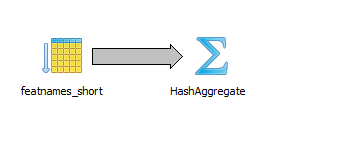
\includegraphics[height=8em]{pg91_btree_explain_like2.png}
\end{center}
\end{columns}
\end{frame}

\section{Conclusion}

\frame{
  \frametitle{Conclusion}

\begin{center}
  SQL fait partie de vos outils de développeur, tirez-en le meilleur!
  \linebreak
  \linebreak

  \begin{center}
    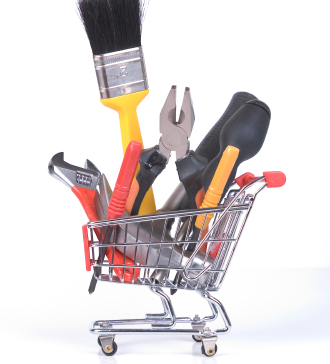
\includegraphics[height=2.1in]{skill-set.jpg}
  \end{center}
\end{center}
}

\end{document}
